\chapter{BioScope: a Flexible and Extensible Wearable Platform}
This chapter presents the design and implementation of BioScope, a flexible and extensible wearable platform for rapidly prototyping healthcare applications. BioScope is an extensible bandage system with components that can be stacked like Lego blocks. Using this system, users can simultaneously collect the four most commonly monitored biosignals (i.e., heart rate, body temperature, acoustic signals emitted from the body, and inertial readings of human movement) from multiple bandages to assess and diagnose physical conditions. BioScope extracts the processing and communication functions into a core building block, and hosts the required sensors. Each sensor is affixed as a patch that collects one biosignal. By stacking the required sensors onto a bandage-like platform, users can easily create a customized bandage that can be affixed to the skin of the patient. The data collected by the sensors are sent through a Bluetooth interface to the device screen used by the healthcare worker. 

\section{BioScope System Design and Implementation}
Based on the design considerations, we designed and implemented the BioScope system. The following subsections include (1) flexible and extensible sensing bandage, (2) stacking mechanism, (3) sensor patches, li4) explorative experiment.

\begin{figure}[!ht]
\centering
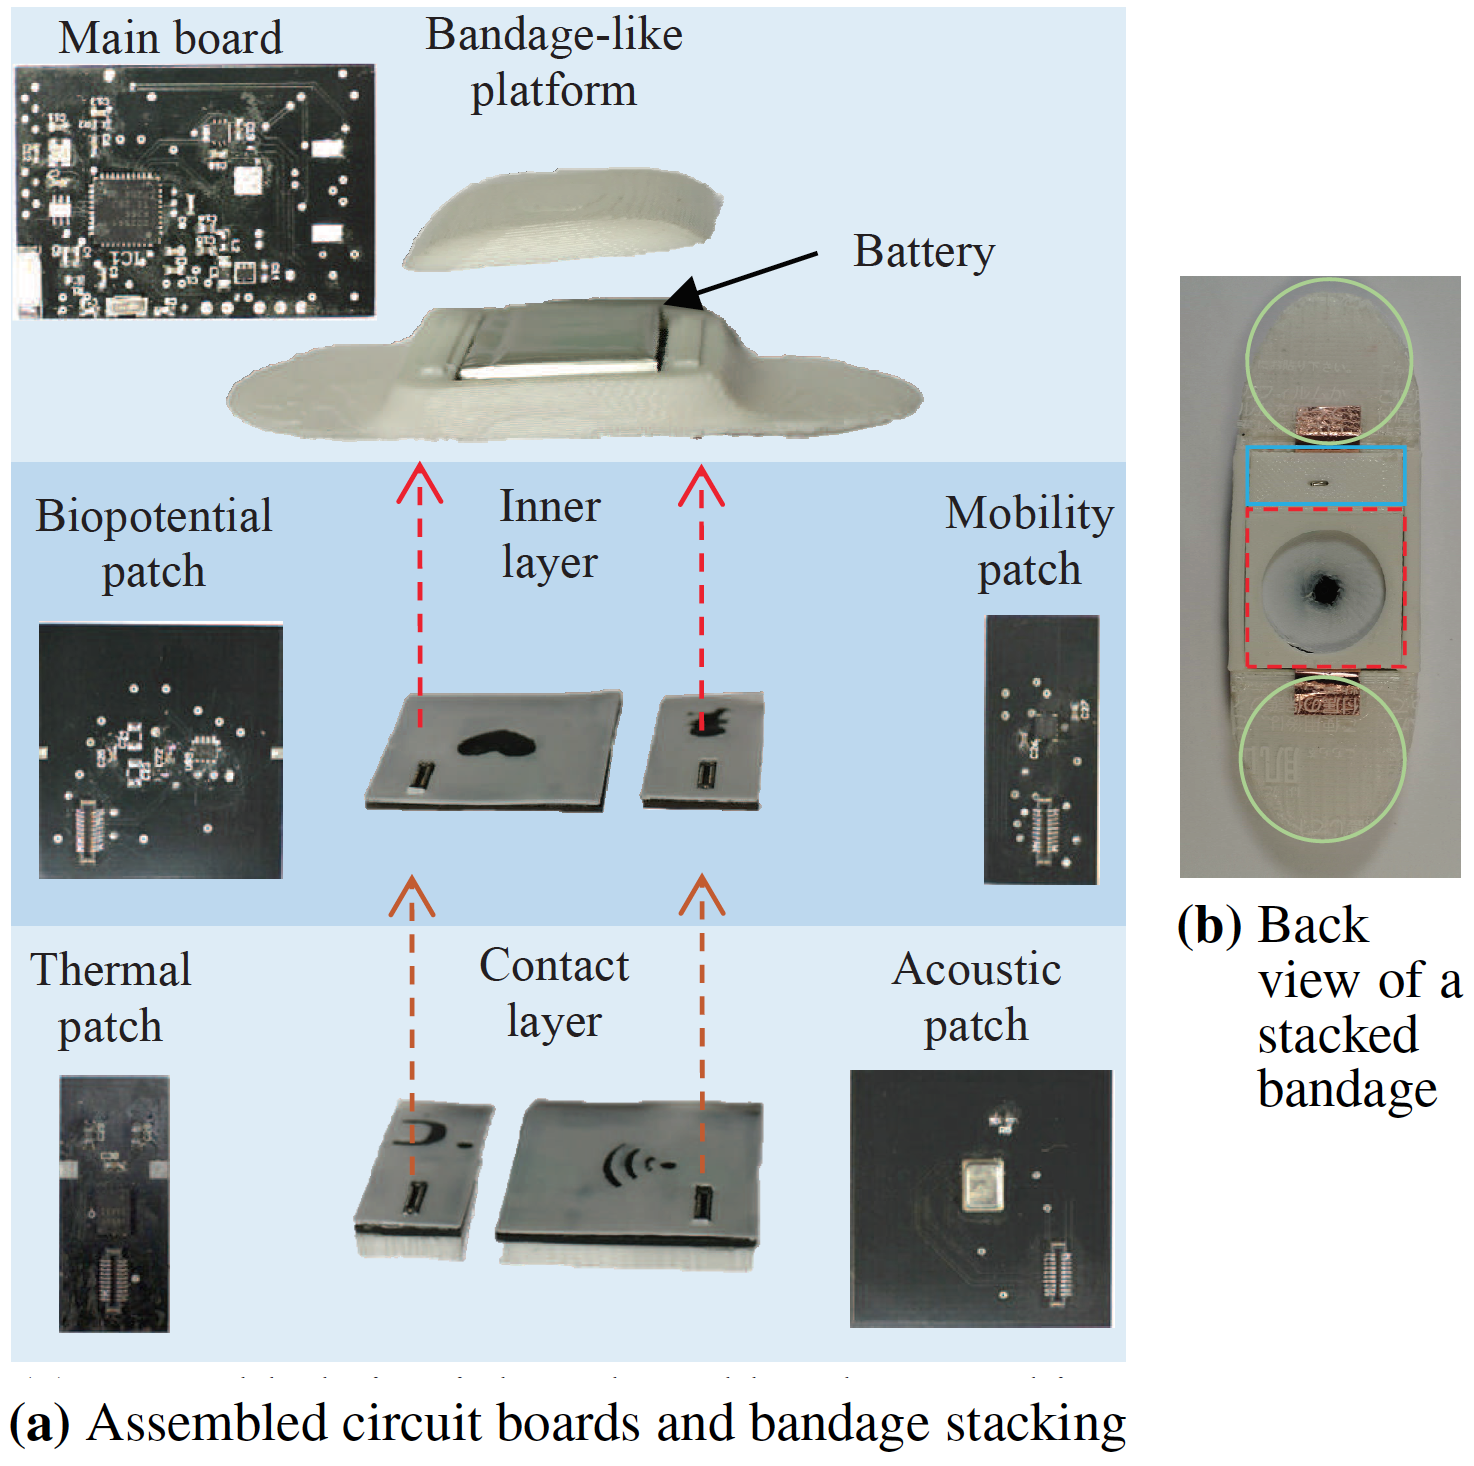
\includegraphics[width=14cm]{image/bio_fig1}
\caption{Design of the extensible sensing bandage. (a) Four patches with distinctive embossed icons are stacked on the inner and contact layers according to the direction indicated by the red dotted arrows. (b) The sound-collecting structure (box with red dashed border), a thermocouple wire (box with blue solid border), and two electrodes coated with a conductive gel (two green circles) directly contact the skin.}
\label{bandage_stacking}
\end{figure}


\subsection{Flexible and Extensible Sensing Bandage}
To create an extensible system, we designed a device with two distinct modules (Figure \ref{bandage_stacking}): (1) the basic bandage platform and (2) sensor patches. The bandage-like platform resembles an adhesive bandage. We drew a 3D model of the platform and then printed it using a 3D printer and elastic filaments. Figure \ref{bandage_stacking}(a) depicts the platform, in which a hollow space is reserved to encase the customized sensing patches. To provide processing and communication capabilities, we designed a customized circuit board, called the main board, that could be mounted in the hollow space. The main board and the stacked sensor patches are powered by a 130-mAh Li-ion battery situated in the upper layer of the platform. On the main board, a Microchip PIC32MX150 microcontroller receives data from the sensor patches through board-to-board connectors, and then relays the processed data to the monitoring screen through a Texas Instruments CC2451 Bluetooth module. \vspace{20pt}

\begin{figure}[!ht]
\centering
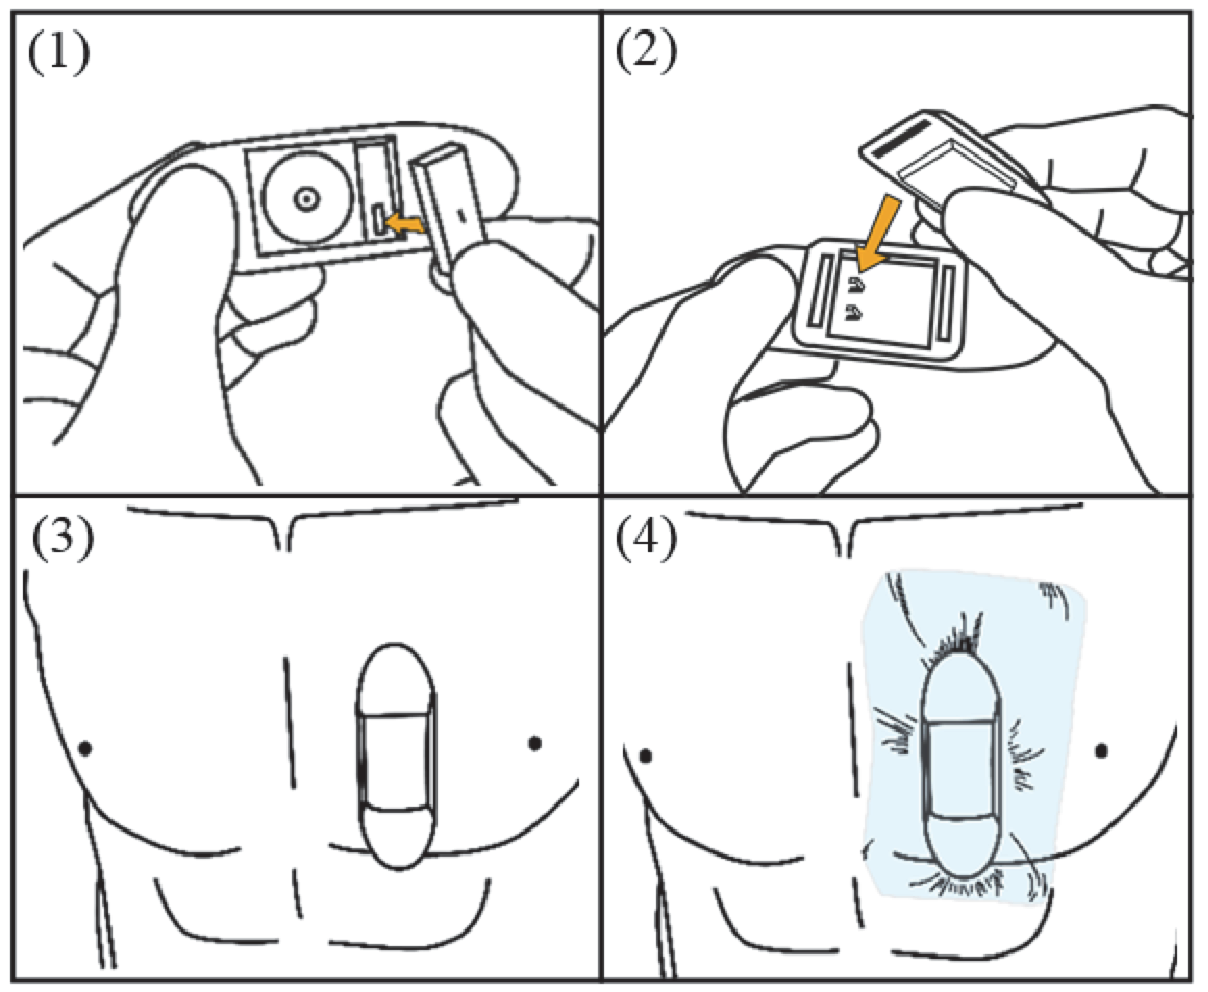
\includegraphics[width=15cm]{image/bio_fig2}
\caption{Four steps for applying bandages.}
\label{bio_steps}
\end{figure}

\subsection{Stacking Mechanism}
Users can choose different combinations of LEGO-like sensing and interaction blocks and assemble them inside a bandage form factor. This subsection describes the three main parts in stacking mechanism to make this system flexible and extensible.

\vspace{15pt}
\textbf{Assembling:}
\newline
Figure \ref{bandage_stacking}(a) illustrates these patches stacked in two layers in the hollow space of the platform; temperature and microphone sensors directly contact the skin to collect high-quality signals. 
To create accessible patches for the users, each patch was punched with a representative icon on both sides of the covering material. Figure \ref{bio_steps} illustrates the BioScope application process: (1) A healthcare worker selects the appropriate patches (or dummy patches) by using the embossed icon as a reference, stacks the patches on (or filling in empty spaces that are originally occupied by unused patches on) the platform, (2) inserts a battery and closes the protection cap, (3) affixes the bandage to chest, and (4) covers the entire bandage with transparent film dressings if water-proof is needed.
\vspace{15pt}
\begin{figure}[ht]
\centering
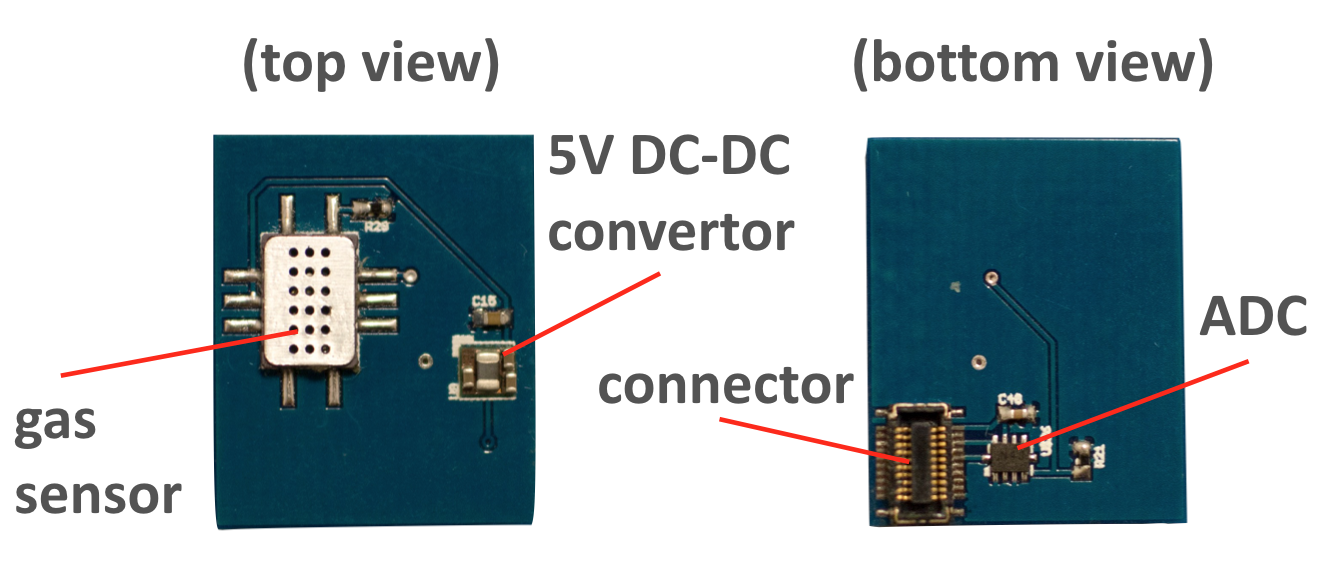
\includegraphics[width=15cm]{image/bio_dc_adc}
\caption{An example of using BioScope to prototype a breathalyzer.}
\label{dc_adc}
\end{figure}
\vspace{5pt}

\vspace{10pt}
\textbf{Power source:}
\newline
Each component in the system has different power supply range. Since  a component may require a supply voltage higher or lower than the voltage from li-ion battery (4.2V), the voltage of power source should be converted to proper voltage. A linear regulator can be used for the component, the working voltage of which is lower than the power source in the system. If the supply voltage of a component is higher than power source, a DC-DC converter can converts the voltage to a higher voltage. In figure \ref{dc_adc}, the supply voltage of the gas sensor is 5V which is higher than the voltage of the battery. Therefore, we place a compact DC-DC convertor, a Texas Instruments TPS81256, to boost the voltage to 5V and provide sufficient current to enable the sensor.

\vspace{10pt}
\textbf{Data communication:}
\newline
For a sensor that communicate to the microcontroller through digital bus, I2C and SPI are two most common protocols. Those protocols is bus topology that allows microcontroller can access multiple slave components with only few pins. However, some sensors are designed to output analog signals to deliver sensory data rather than digital signals. In Figrue \ref{dc_adc}, a Texas Instruments ADS1114 analog-to-digital converter translates the analog signals from gas sensor to digital signals in I2C.

\subsection{Sensor Patches}
To collect biosignals, such as electrocardiogram (ECG) signals, two pre-allocated electrodes (i.e., two conductive copper areas situated 6.4 cm apart at opposite ends of the bandage) are coated with a thin layer of electrical gel (Figure \ref{bandage_stacking}(b)).
The sensor patches, consisting of small sensor boards sandwiched between two thin layers of 3D-printed elastic filaments, are mounted on the bandage-like platform using connectors. To demonstrate the concept of this system, we designed six types of patch — biopotential, thermal, acoustic, mobility, interaction and recharging patches — to facilitate the collection in the most commonly monitored data in healthcare applications.
The detail of those six types of patch are described in follows.
\vspace{15pt}
\newline 
\textbf{Biopotential patch:}
\newline
This 23 mm × 24 mm patch, stacked in the inner layer, amplifies and filters ECG signals to enable continual cardiovascular monitoring. Cardiac activity, which can be characterized by ECG signals, is a crucial biosignal for assessing the cardiac functions of people. By amplifying the electrical potential difference measured between the two electrodes by using a Texas Instruments ADS1115 analog-to-digital converter on the patch, ECG signals can be monitored by allowing the passing of low-frequency signals from 0 to 100 Hz \cite{shaikh1995} by using a low-pass filter. A pulse can be identified by detecting spikes in the signal, thus enabling users to assess heart and respiratory rates.
\vspace{10pt}
\newpage
\textbf{Acoustic patch:}
\newline
This 24 mm × 24 mm patch, stacked in the contact layer, records acoustic signals emitted by a person's body or while the person is phonating. By identifying the unique sound patterns that the body's organs generate, users can assess person's conditions. Furthermore, person's phonation can indicate social interaction, according to which users can assess whether a person is depressed or impaired cognitively.  To clearly record the internal sounds of the body, a mediating instrument (e.g., a stethoscope) is required. Inspired by the design of electronic stethoscopes, we designed and attached a small sound-collecting structure (Figure \ref{bandage_stacking}(b)) on the patch that effectively amplified acoustic signals from the body and occluded environmental noise. Above the sound-collecting structure, an opening is aligned with the receiving hole of an InvenSense INMP441 microphone on the main board to guide sound waves towards the hole. In this study, we detected a person phonation, which reflected social activity, by analyzing the frequency components of the collected sound.
\vspace{10pt}
\newline
\textbf{Thermal patch:}
\newline
This 10 mm × 24 mm patch is stacked in the contact layer and measures the skin temperature, which can indicate a person's health. users can evaluate a person by identifying abnormal or varying temperatures \cite{Freitas1999}. A Maxim MAX31850 K-type thermocouple-to-digital converter detects body temperature through a thermocouple wire that protrudes from the covering elastic material to contact the skin of the person (Figure \ref{bandage_stacking}(b)).
\vspace{10pt}
\newpage
\textbf{Mobility patch:}
\newline
This 11 mm × 24 mm patch, stacked in the inner layer, monitors the mobility level of a person. For example, to prevent complications caused by reduced mobility levels and assess functional recovery, users must track the mobility level of patients. On this patch, a Bosch BMA250 accelerometer is used to collect acceleration readings, which indicate whether a person is moving or stationary. The mobility level can be derived by calculating the percentage of time a person is moving.
\vspace{10pt}
\begin{figure}[ht]
\centering
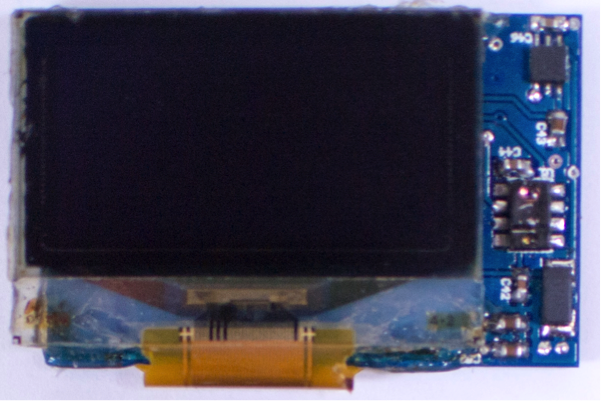
\includegraphics[width=12.5cm]{image/bio_fig1_5}
\caption{Interaction patch.}
\label{interaction_patch}
\end{figure}
\newline
\textbf{Interaction patch:}
\newline
To enrich data feedback and user interaction for exercise applications, we also expanded an interaction patch that consists of a wearable display (0.96” OLED display4), and a touchless gesture sensor (Avago APDS-9960) that is used to recognize four directions (up, down, left and right) of in-air swipe gesture. The gesture can be used to switch between different sensor's data or different data representations as shown in Figure \ref{interaction_patch}. The interaction patch is connected to main board through stacking mechanism as well. When a mobile device attempts to establish connection with particular one of multiple wearable devices. To simplify Bluetooth pairing procedure for quickly retrieving data or configuring device, a NXP NTAG203 NFC tag is embedded in wearable device.
\vspace{10pt}
\begin{figure}[ht]
\centering
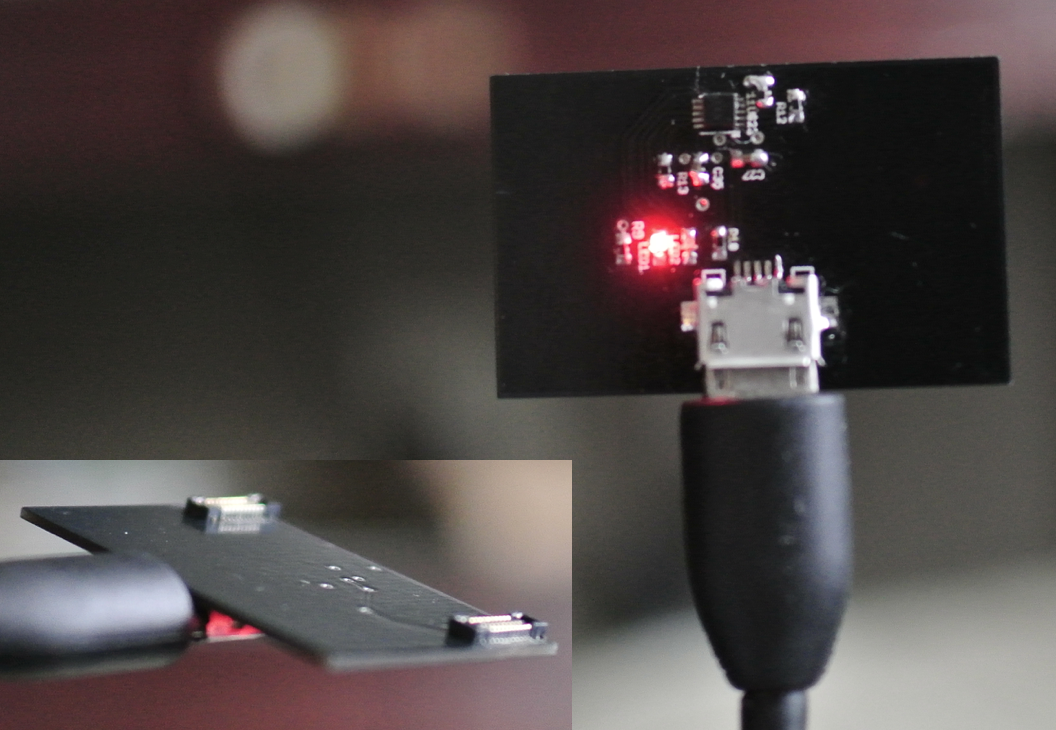
\includegraphics[width=13cm]{image/bio_recharge}
\caption{Recharging patch.}
\label{bio_recharge}
\end{figure}
\newline
\textbf{Recharging patch:}
\newline
The entire system is powered by a Li-ion battery with 130-mAh capacity. This patch has a USB connector to connect a 5V power source for charging and a Texas Instruments BQ24040 to regulate the voltage in charging process (Figure \ref{bio_recharge}).


\subsection{Explorative Experiment}
To validate system functionality, we scripted a sequence of activities to simulate conditions arising when a patient with basic functional mobility is hospitalized. Two volunteers performed the specific activities while wearing bandages equipped with all four patches on their chests, enabling us to collect data (Figure \ref{bio_exp_result}(a)). The simulations were con- ducted for 10 and 30 minutes in the cases of the first and second participants (P1 and P2), respectively. Activities comprised (1) lying down on a bed, (2) having a phone conversation, (3) watching TV, (4) having a face-to-face conversation, and (5) performing walking. In the experiments, the data captured were heart rate, skin temperature, received acoustic signals, and mobility indicators.

Figure \ref{bio_exp_result}(b) shows the results obtained by analyzing the data collected from P1. The readings obtained from the mobility patch indicated that P1 moved between the seventh and ninth minutes; this was an accurate assessment of the patient's behavior during that time. While walking, P1's heart rate increased relative to that while stationary between the start and the seventh minute. When the posture of the patient drastically changed, such as when P1 stood up near the second, seventh, and ninth minutes, the ECG signals were distorted \cite{chan2013}, producing a dip in the calculated heart rate. The sounds generated by clothes rubbing against the bandage when P1 moved adversely affected the quality of detected internal sounds, causing the amplitudes to increase between the seventh and ninth minutes. After filtering out sounds generated by movement, however, we could still detect when P1 phonated between the second and seventh minute. Based on the vocal resonance of the body \cite{Dacre2002}, we detected phonation by identifying the frequency components of sounds higher than the 0- to 3-kHz frequency range of the human voice [7]. Finally, the body temperature varied minimally (34$^{\circ}$C $\sim$ 35$^{\circ}$C) and was near the normal skin temperature of the human chest \cite{Freitas1999}. Overall, the results accurately reflected the activities performed by the participants.

To examine whether the system can detect reasonable values for the average heart rate, total moving duration, average skin temperature, and total phonating time, we analyzed the data collected from P2 over 30 minutes. The total moving duration was determined to be 7.2 minutes (actual value: 6.9 minutes), with an error of 4.0\%. The average heart rate was 81.5 and 100.3 beats respectively.  Because P2 did not perform intensive exercise, the average temperature did not vary significantly, remaining near 33.9◦C. By identifying the high-frequency components embedded in the high-pitched sounds collected when P2 was stationary, P2 was deter- mined to have phonated for 635.5 seconds (actual value: 564.0 seconds), with an error of 12.7\%. per min (BPM) when P2 was stationary and moving, respectively.  Because P2 did not perform intensive exercise, the average temperature did not vary significantly, remaining near 33.9◦C. By identifying the high-frequency components embedded in the high-pitched sounds collected when P2 was stationary, P2 was deter- mined to have phonated for 635.5 seconds (actual value: 564.0 seconds), with an error of 12.7\%.

\begin{figure}[!ht]
\centering
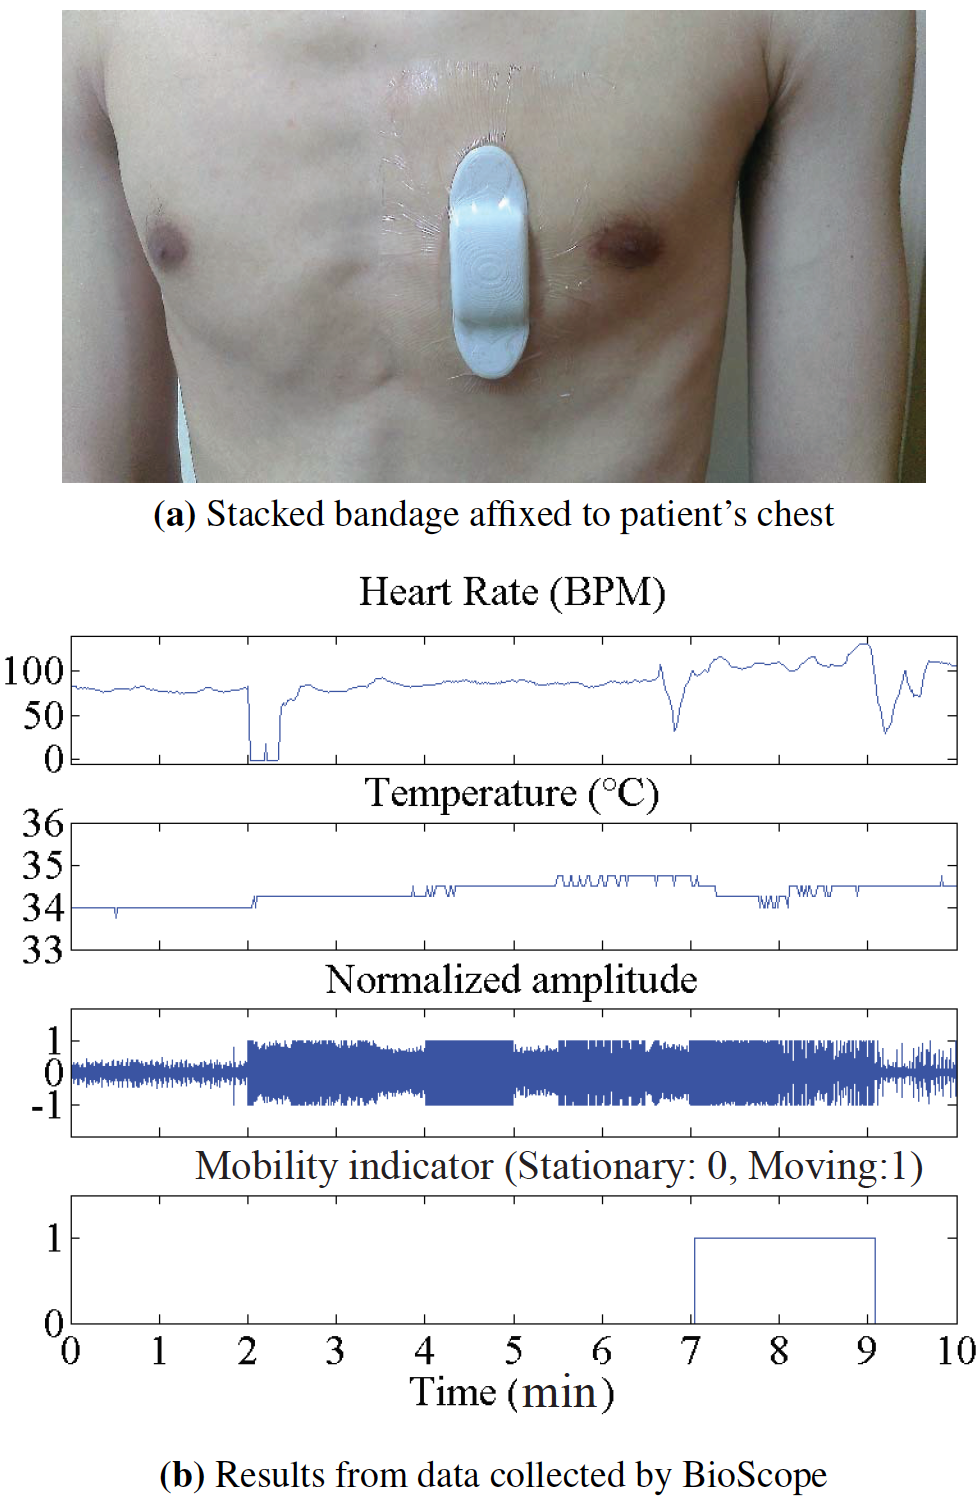
\includegraphics[width=12cm]{image/bio_fig4}
\caption{Four steps for applying bandages.}
\label{bio_exp_result}
\end{figure}


%\section{Configuration}

%\section{Application programming interface}

\section{...}


\section{...}

